\documentclass[10pt]{article}

\usepackage[a4paper, left=2cm, right=2cm]{geometry} % A4 paper size and thin margins

\usepackage{xcolor} % Required for specifying custom colours
\definecolor{grey}{rgb}{0.9,0.9,0.9} % Colour of the box surrounding the title

\usepackage{graphicx}
\usepackage[colorlinks=true, allcolors=black]{hyperref}
\usepackage{amsmath}
\usepackage{indentfirst}
\usepackage{float}
\setlength{\parindent}{2em}


\usepackage[utf8]{inputenc} % Required for inputting international characters
\usepackage[T1]{fontenc} % Output font encoding for international characters
\usepackage[sfdefault]{ClearSans} % Use the Clear Sans font (sans serif)
%\usepackage{XCharter} % Use the XCharter font (serif)
\newcommand{\tabincell}[2]{\begin{tabular}{@{}#1@{}}#2\end{tabular}} 	


\begin{document}
%----------------------------------------------------------------------------------------
%	TITLE PAGE
%----------------------------------------------------------------------------------------

\begin{titlepage} % Suppresses displaying the page number on the title page and the subsequent page counts as page 1
	
	%------------------------------------------------
	%	Grey title box
	%------------------------------------------------
	
	\colorbox{grey}{
		\parbox[t]{1.1\textwidth}{ % Outer full width box
			\parbox[t]{1.02\textwidth}{ % Inner box for inner right text margin
				\raggedleft % Right align the text
				\fontsize{34pt}{40pt}\selectfont % Title font size, the first argument is the font size and the second is the line spacing, adjust depending on title length
				\vspace{0.7cm} % Space between the start of the title and the top of the grey box
				
				< Journey Assistant >\\
                Software Architecture Document\\
                Version 1.0\\
				
				\vspace{0.7cm} % Space between the end of the title and the bottom of the grey box
			}
		}
	}
	
	\vfill % Space between the title box and author information
	
	%------------------------------------------------
	%	Author name and information
	%------------------------------------------------
	
	\parbox[t]{1\textwidth}{ % Box to inset this section slightly
		\raggedleft % Right align the text
		\large % Increase the font size
		{\Large Group Member}\\[4pt] % Extra space after name
        Yiwen Song\\
        Zhihui Xie\\
        Weizhe Wang\\
        Huangfei Jiang\\
        Haoping Chen\\
		% Institution Name\\[4pt] % Extra space before URL
		% \texttt{LaTeXTemplates.com}\\
		
		\hfill\rule{0.2\linewidth}{1pt}% Horizontal line, first argument width, second thickness
    }
    
	
\end{titlepage}

\newpage

\begin{center}
    {\LARGE Modification History}
    
    \begin{tabular}{|c|c|c|c|} 
        \hline 
        Date&Version&Description&Author\\
        \hline  
        2019-04-16&1.0&The first version of this document.&Zhihui Xie \& Yiwen Song\\
		\hline 
		 & & & \\
		\hline
		& & & \\
		\hline
		& & & \\
		\hline
    \end{tabular}    
\end{center}

\newpage

\tableofcontents
\newpage

\section{Introduction}
\subsection{Purpose}
The purpose of this software architecture document is to make clear the architecture of our software, and lead the development team to develop the software according to our architecture.

The intended readers of this document is the developers of the software.


\subsection{Scope}
This document will be applied in our software development, particularly Journey Assistant. We don’t intend to apply this document on any other software under development.

\subsection{Definition}
Here we list some terms or abbreviations we will use in this file.

\begin{table}[htb]
	\centering
	\begin{tabular}{|c|c|c|} 
		\hline 
		Abbreviation&Term&Implication\\
		\hline  
		JA&Journey Assistant&The Name of our Project\\
		\hline 
		 &Android&An OS Developed by Google\\
		\hline
		IM&Instant Messaging&\tabincell{c}{A type of online chat that offers real-time \\ text transmission over the Internet}\\
		\hline
	\end{tabular}    

	\caption{Terms or Abbreviations}\label{Terms or Abbreviations}
\end{table}

\section{Architecture of the Current System}
The architecture of the current software system is shown below (Figure \ref{Architecture of Current System}). We can see that the current system don’t have a multi-functional architecture and it needs human service to complete the task.

Therefore, what we will do to improve the system is to change the human service into automative service, and make the system more complete.

\begin{figure}[H]
	\centering
	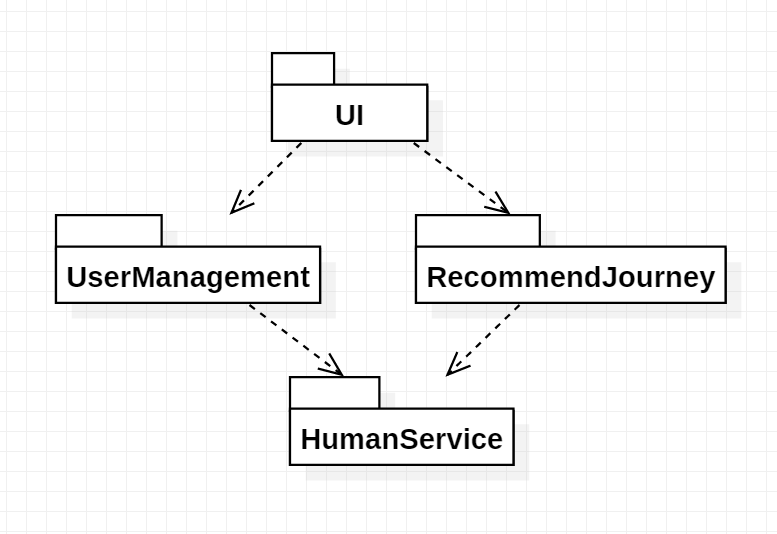
\includegraphics[width=14cm]{current.png}
	\caption{Architecture of the Current System}
	\label{Architecture of Current System}
\end{figure}

\section{Design Objective of System Architecture}
The following requirements and goals of our software has great influence on our software architecture:

\begin{itemize}
	\item[(1)]The security of our software. We need to make sure that all the information in our software system are kept securely, especially the personal information of our users. Therefore, we must add components in our architecture to ensure the security of our software.
	\item[(2)]The synchronization of information. The user-provided information and the information we provided to the users should be synchronized on our server. Given the user’s account, the server should be able to recover all information provided by the user and recent information we have provided to the user, in case the user re-install the software.
	\item[(3)]The extension-support. At the beginning of our software, we do not consider using high-level hardware. However, when the user crowd has grown to a certain level, our system would be able to be transferred to a higher-level harware server easily.
	\item[(4)]High-proficiency level. Our system should be able to react quickly and accurately to the users’ various queries. 
	\item[(5)]High capatibility. Our system should be able to run on different versions of Andriod operating systems, or at least run on Android version 6.0, 7.0 and 8.0, which is widely used currently.
\end{itemize}

\section{Architecture of our Proposed System}
\subsection{Introduction}

\begin{itemize}
	\item[(1)] We use client/server architecture as our main system architecture.

	The system is devided into the frontend client and backend server. The frontend is the application of users' cellphones, and the backend is the server that achieves system functionality and saves data.

	The reason why we choose client/server architecture is that the architecture is mature and has been widely used in this kind of service application developments. It also helps the centered management of data, while our system is data-centered.

	\item[(2)] We use 3-layered architecture as our subsystem architecture.

	We use 3 layers to organize our subsystems. The first layer is user-interface layer, which provides the port for user interface. The second layer is application logic layer, which is in charge of controling and realizing system functionality. The third layer is web-service layer, which is in charge of the web service of data tranmission.

	The 3-layered architecture is mature. It devides the port and the logic layer apart, leading to a low-coupling system, making our system easier to extend and maintain.

	\item[(3)] We use MVC as our model architecture.
 
	The MVC model fits well with our interaction system. We have devided the system into three layers, so it's easy for us to do MVC separation.
	
\end{itemize}

\textbf{The system includes the following subsystems:}

\paragraph{\underline{UI}} In charge of the interaction between the system and users.

\paragraph{\underline{UserManagement}} In charge of management of user information, including “login”, “sign in”, and “change information” instructions.

\paragraph{\underline{JourneyManagement}} In charge of making plans about itinerary and making simulations given journey details.

\paragraph{\underline{ReportManagement}} In charge of handling report from users.

\paragraph{\underline{CommonService}} In charge of data I/O, the communication between the client and the server.

\subsection{Use Case View}
\begin{figure}[H]
	\centering
	
	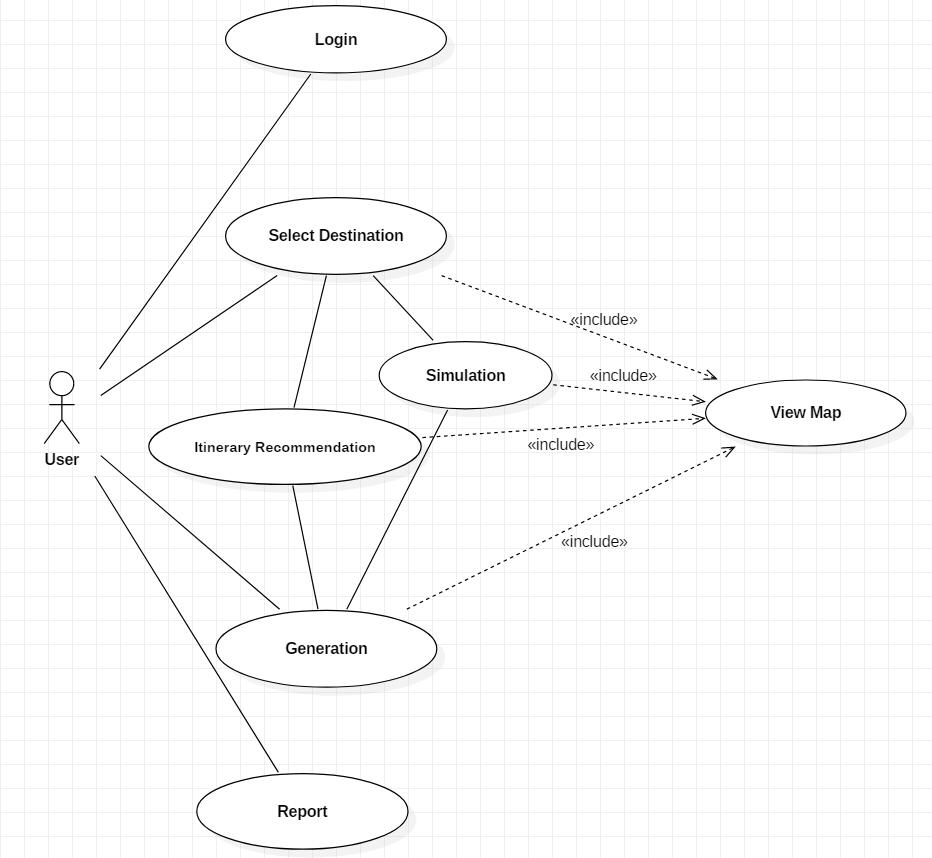
\includegraphics[width=14cm]{usecase.jpg}
	\caption{Use Case View}
	\label{Use Case View}
\end{figure}

\subsection{Logic View}
\subsubsection{System Architecture}
The system architecture diagram is shown in the following figure. The whole system in devided into 7 sub-systems, respectively UI, UserManagement, DataManagement, DialogManagement, SimulationService, RecommendationService, and CommonService. Each subsystem will be introduced later.

\begin{figure}[H]
	\centering
	
	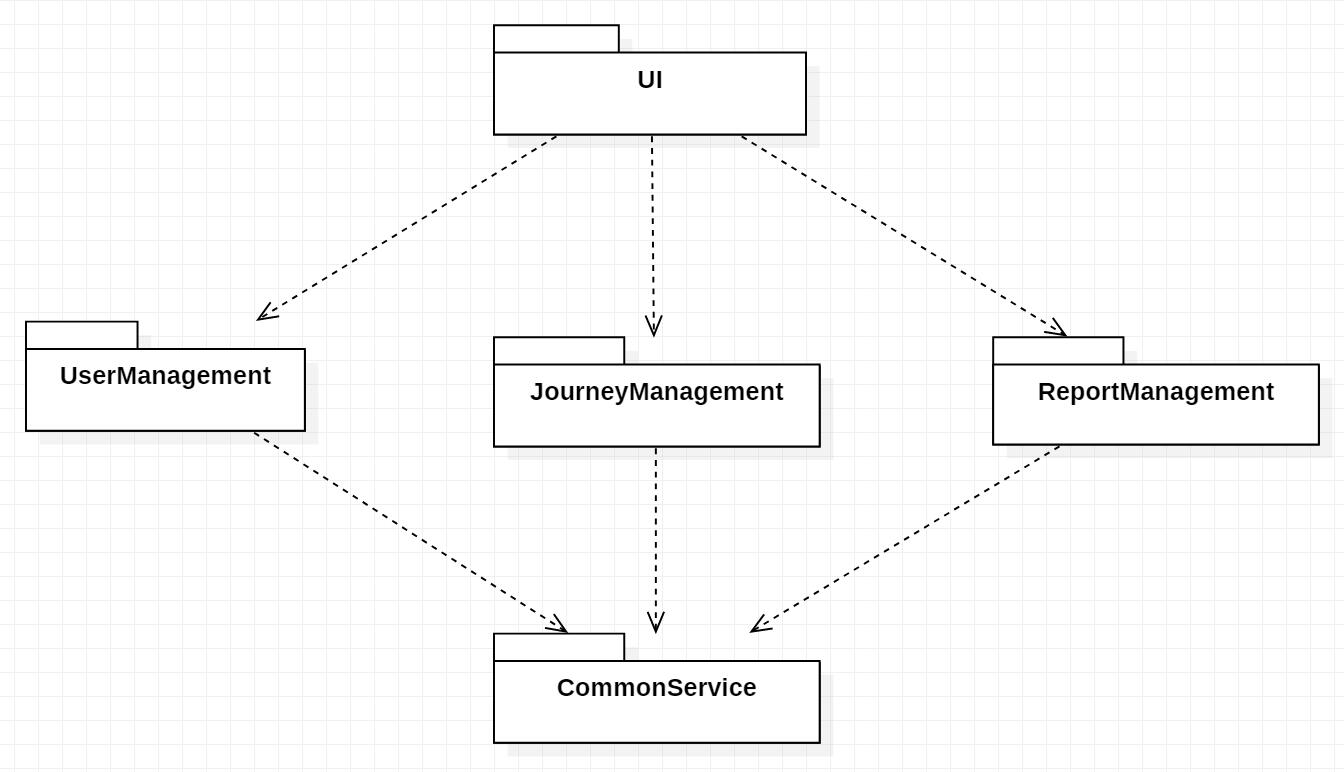
\includegraphics[width=14cm]{architecture.jpg}
	\caption{System Architecture}
	\label{System Architecture}
\end{figure}

The following class diagrams (Figure \ref{UI Subsystem} - \ref{Report Management Subsystem}) show inner logic for every package.

\begin{figure}[H]
    \centering
    
    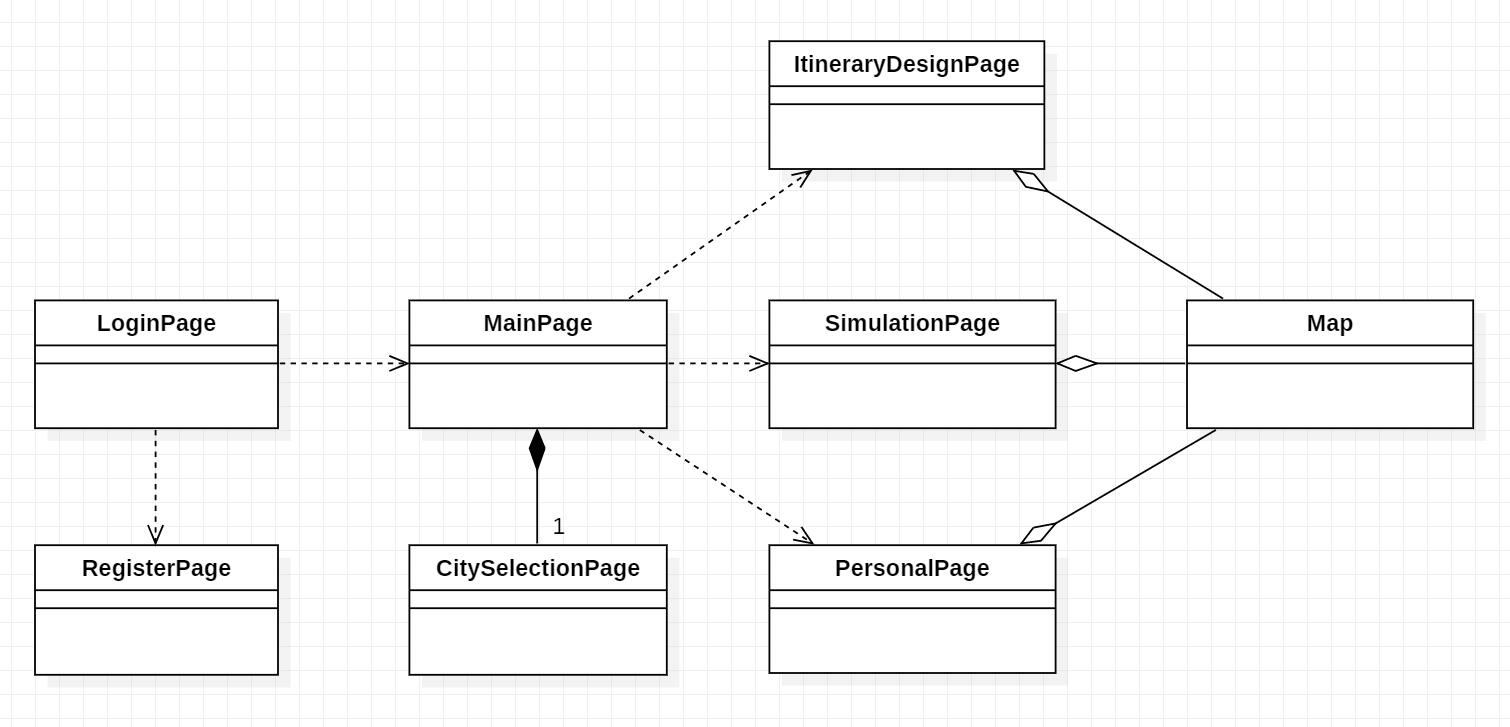
\includegraphics[width=14cm]{ui.jpg}
    \caption{UI Subsystem}
    \label{UI Subsystem}
\end{figure}

\begin{figure}[H]
    \centering
    
    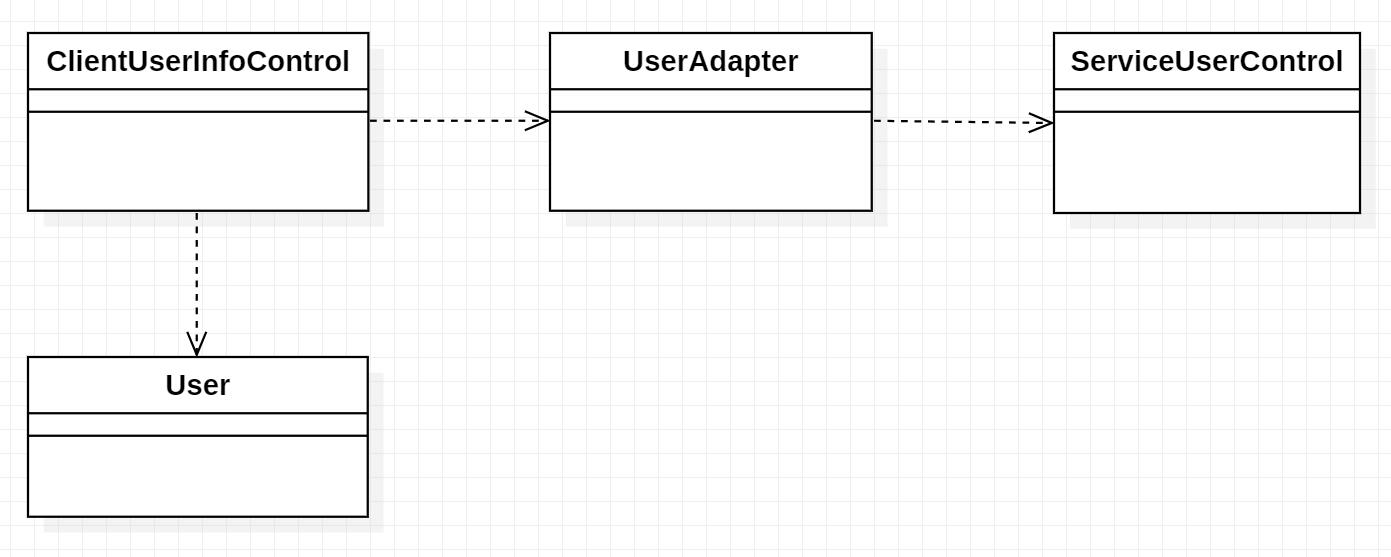
\includegraphics[width=14cm]{usermanager.jpg}
    \caption{User Management Subsystem}
    \label{User Management Subsystem}
\end{figure}

\begin{figure}[H]
    \centering
    
    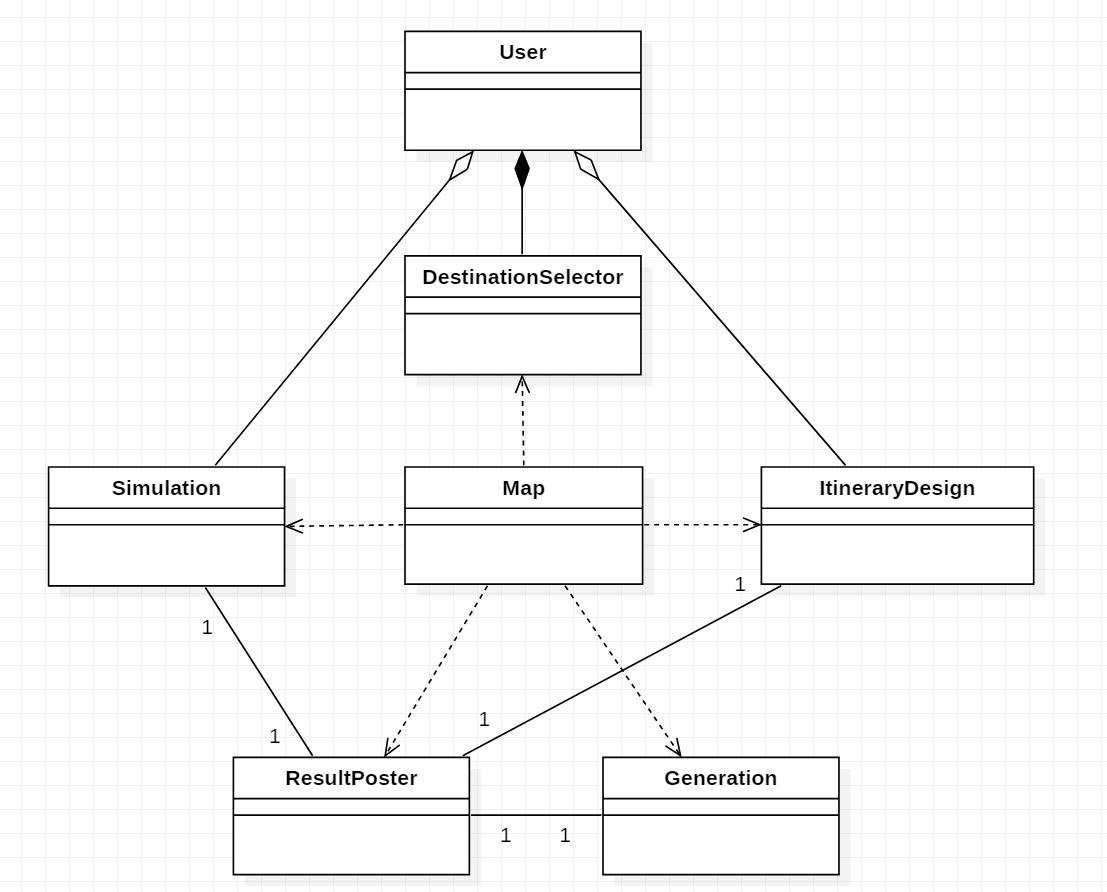
\includegraphics[width=14cm]{journeymanager.jpg}
    \caption{Journey Management Subsystem}
    \label{Journey Management Subsystem}
\end{figure}

\begin{figure}[H]
    \centering
    
    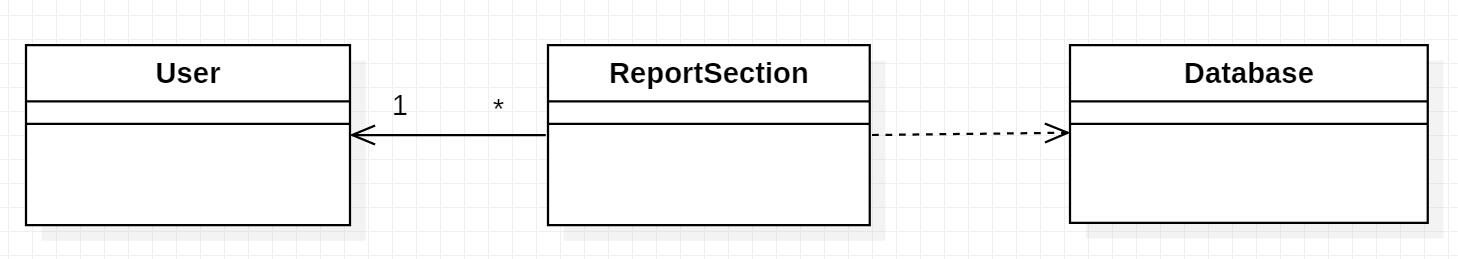
\includegraphics[width=14cm]{reportmanager.jpg}
    \caption{Report Management Subsystem}
    \label{Report Management Subsystem}
\end{figure}

\subsubsection{Subsystem}
Our whole system is composed of 5 subsystems, including the UI subsystem, the UserManagement subsystem, the JourneyManagement susbsystem, the ReportManagement subsystem, and the CommonService subsystem. The detailed ports and the components of the subsystems will be introduced in the following part.

\paragraph{\underline{UI Subsystem}}
\subparagraph{Functionality} The interaction between the system and users.

\subparagraph{Service} UI will provide the input/output box, buttons, frames to support I/O of the messages.

\subparagraph{Class Diagram} Figure \ref{UI Subsystem Class Diagram}
\begin{figure}[H]
	\centering
	
	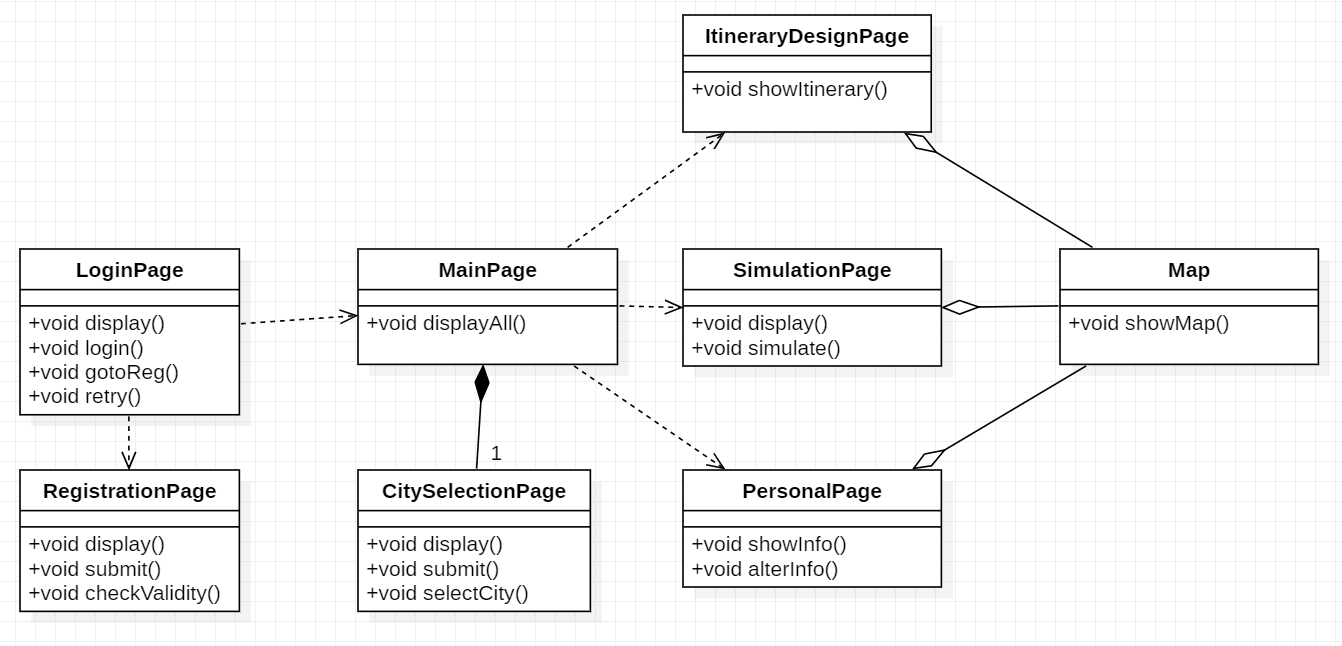
\includegraphics[width=14cm]{uiclass.png}
	\caption{UI Subsystem Class Diagram}
	\label{UI Subsystem Class Diagram}
\end{figure}

\paragraph{\underline{UserManagement Subsystem}}
\subparagraph{Functionality} Management of user information, including “login”, “sign in”, and “change information” instructions.

\subparagraph{Service}  registration, submitUserInfo, login, showPersonalInfo, updatePersonalInfo

\subparagraph{Class Diagram} Figure \ref{UserManagement Subsystem Class Diagram}

\begin{figure}[H]
	\centering
	
	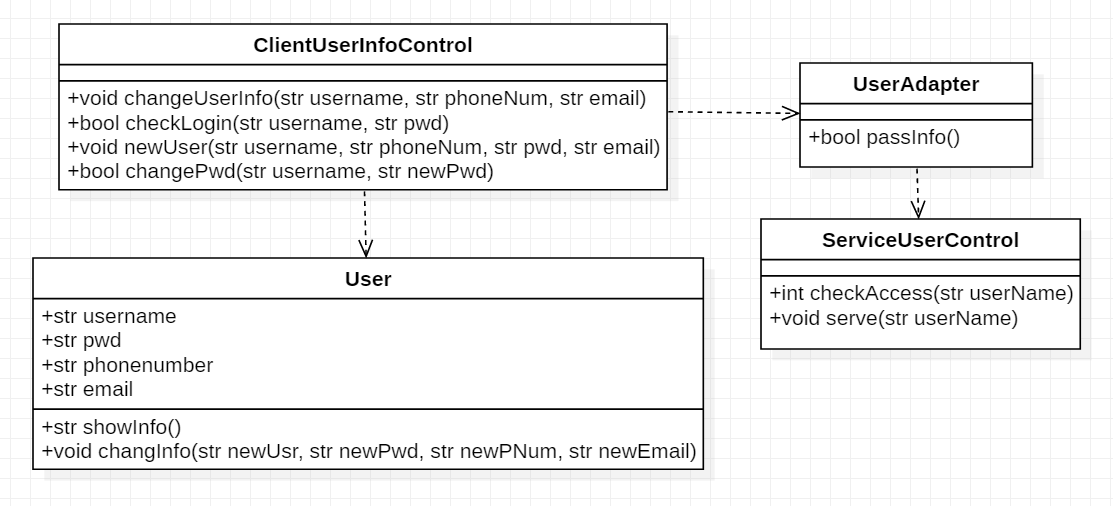
\includegraphics[width=14cm]{usermanageclass.png}
	\caption{UserManagement Subsystem Class Diagram}
	\label{UserManagement Subsystem Class Diagram}
\end{figure}

\subparagraph{Component Diagram} Figure \ref{UserManagement Subsystem Component Diagram}

\begin{figure}[H]
	\centering
	
	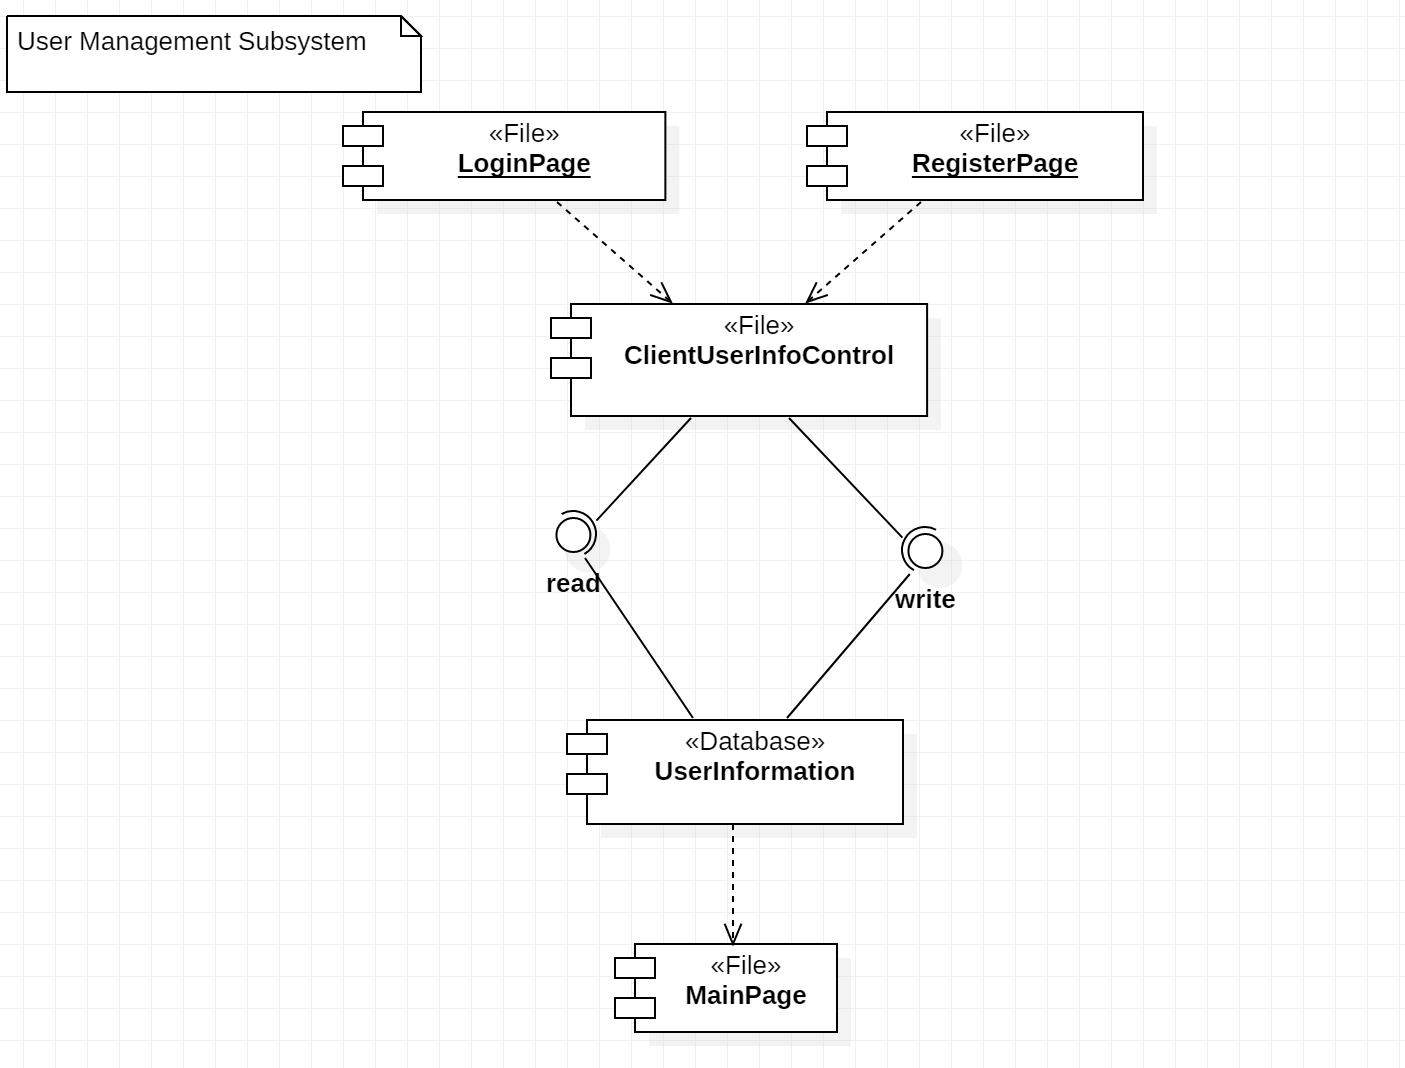
\includegraphics[width=14cm]{usermanagecom.png}
	\caption{UserManagement Subsystem Component Diagram}
	\label{UserManagement Subsystem Component Diagram}
\end{figure}

\paragraph{\underline{JourneyManagement Subsystem}}
\subparagraph{Functionality} Making plans about itinerary and making simulations given journey details.

\subparagraph{Service}  designItinerary, changeItinerary, simulateJourney, selectDestination, showResult, generateResult

\subparagraph{Class Diagram} Figure \ref{JourneyManagement Subsystem Class Diagram}

\begin{figure}[H]
	\centering
	
	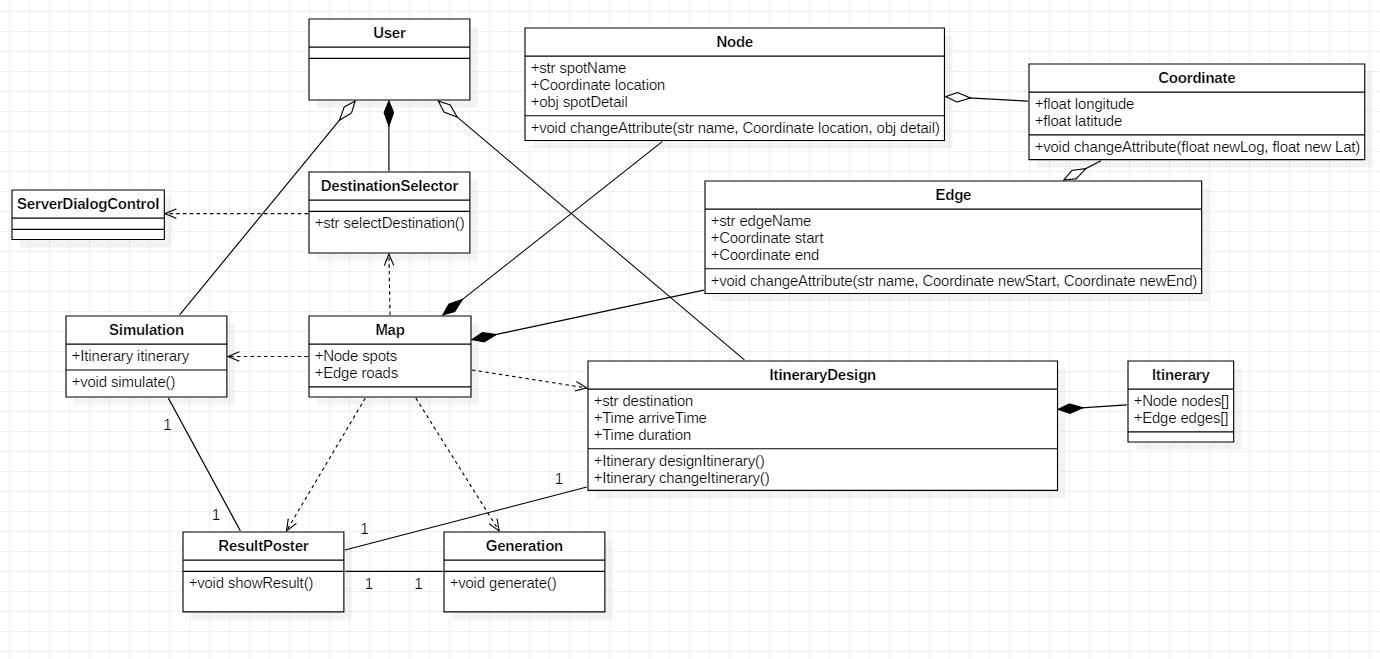
\includegraphics[width=14cm]{journeyclass.png}
	\caption{JourneyManagement Subsystem Class Diagram}
	\label{JourneyManagement Subsystem Class Diagram}
\end{figure}

\subparagraph{Component Diagram} Figure \ref{JourneyManagement Subsystem Component Diagram}

\begin{figure}[H]
	\centering
	
	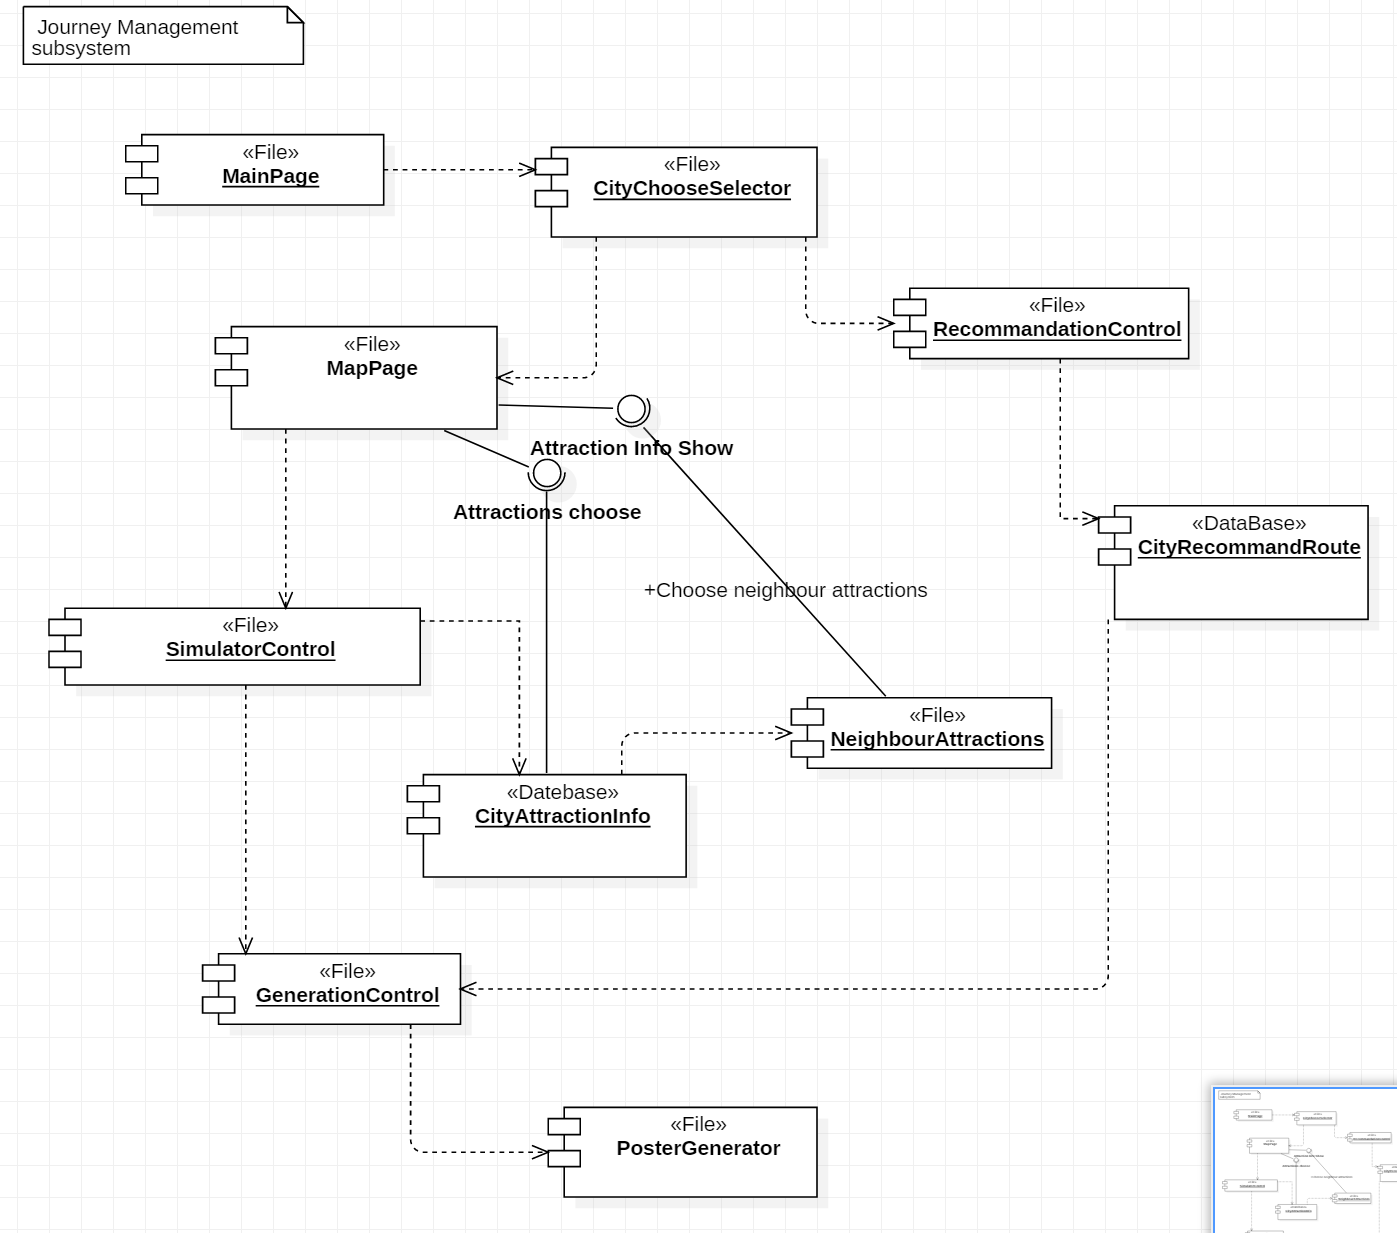
\includegraphics[width=14cm]{journeycom.png}
	\caption{JourneyManagement Subsystem Component Diagram}
	\label{JourneyManagement Subsystem Component Diagram}
\end{figure}

\paragraph{\underline{ReportManagement Subsystem}}
\subparagraph{Functionality} Handle report from users.

\subparagraph{Service}  reportIssue

\subparagraph{Class Diagram} Figure \ref{ReportManagement Subsystem Class Diagram}

\begin{figure}[H]
	\centering
	
	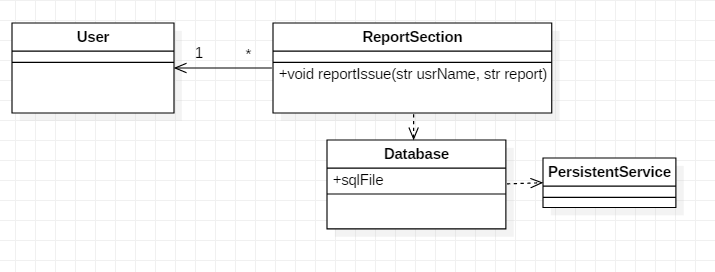
\includegraphics[width=14cm]{reportclass.png}
	\caption{ReportManagement Subsystem Class Diagram}
	\label{ReportManagement Subsystem Class Diagram}
\end{figure}

\subparagraph{Component Diagram} Figure \ref{ReportManagement Subsystem Component Diagram}

\begin{figure}[H]
	\centering
	
	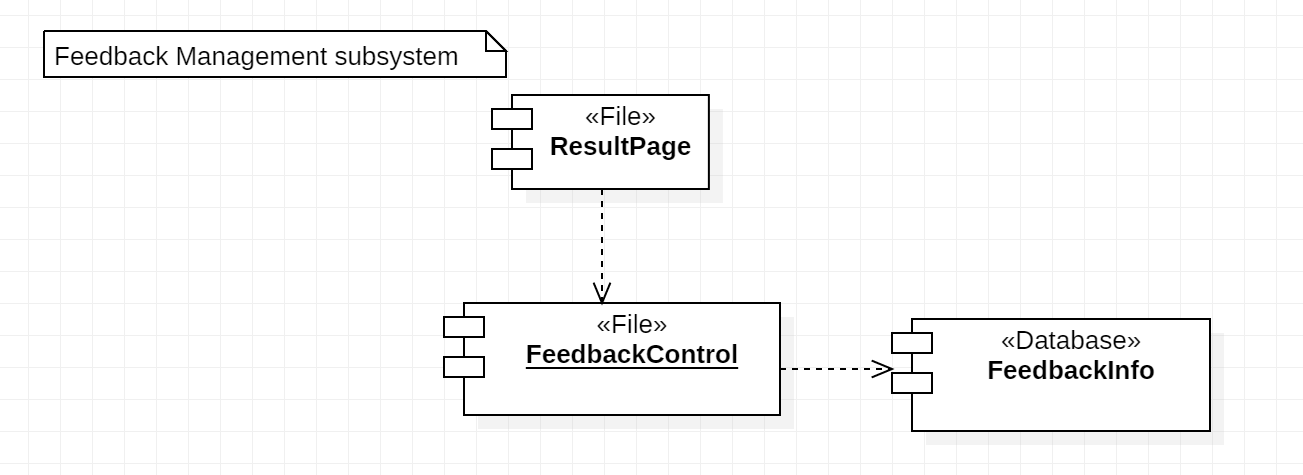
\includegraphics[width=14cm]{reportcom.png}
	\caption{ReportManagement Subsystem Component Diagram}
	\label{ReportManagement Subsystem Component Diagram}
\end{figure}

\paragraph{\underline{CommonService  Subsystem}}
\subparagraph{Functionality} Data I/O, the communication between the client and the server

\subparagraph{Service}  request, startCommunication, sendMsg.

\subparagraph{Class Diagram} Figure \ref{CommonService Subsystem Class Diagram}

\begin{figure}[H]
	\centering
	
	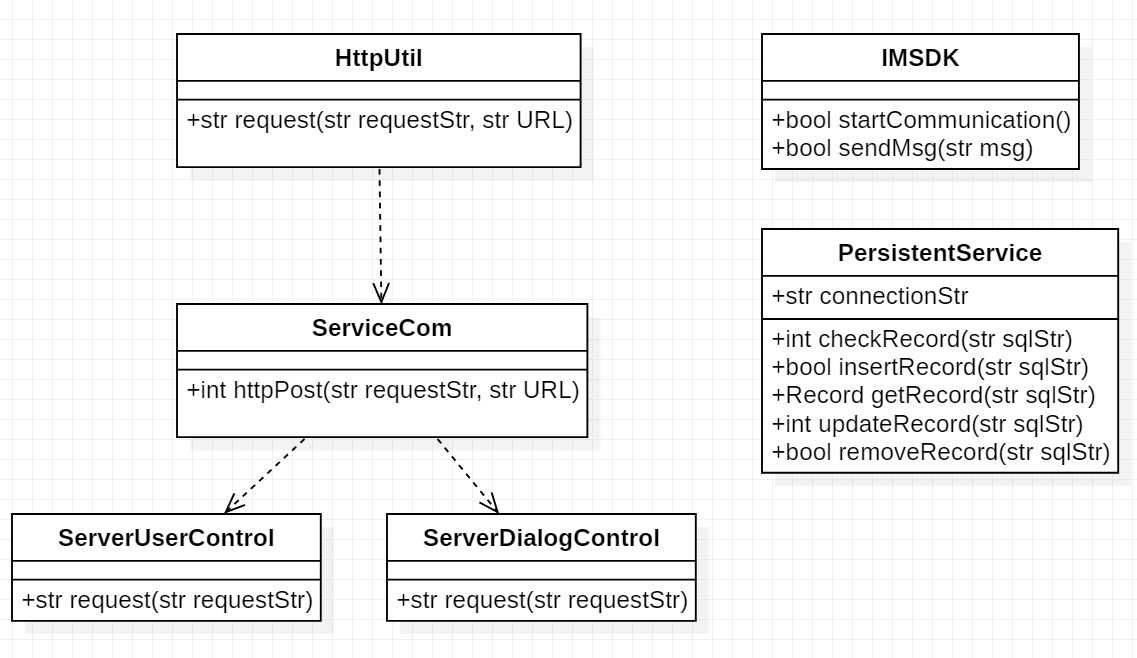
\includegraphics[width=14cm]{commonclass.png}
	\caption{CommonService Subsystem Class Diagram}
	\label{CommonService Subsystem Class Diagram}
\end{figure}

\subsubsection{Use Case Realization}
For each type of use case, we use an interaction diagram to display our corresponding inner design.

\begin{figure}[H]
    \centering
    
    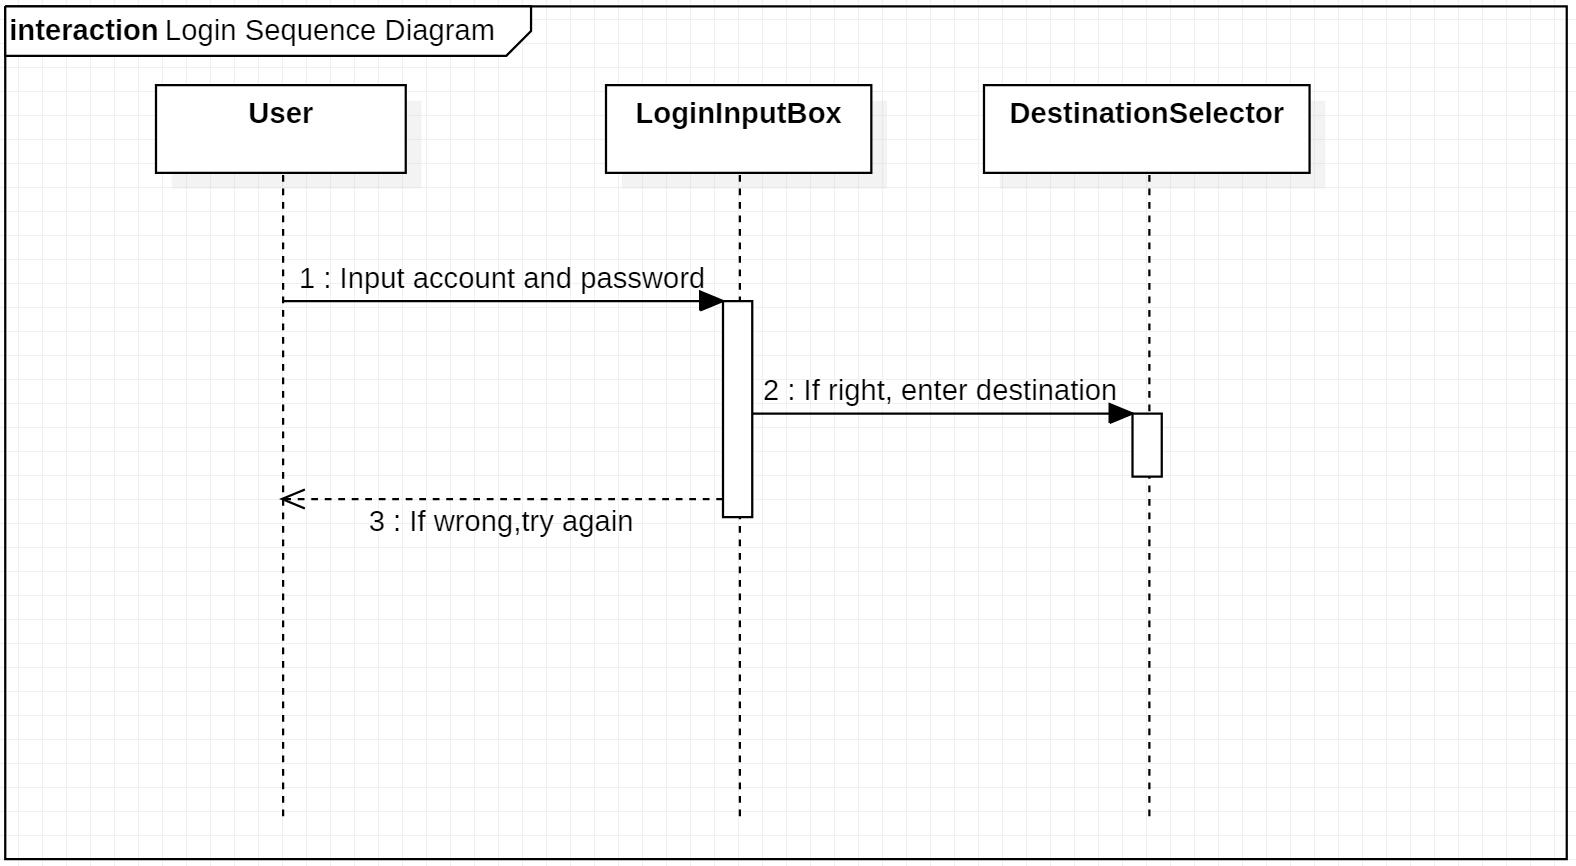
\includegraphics[width=14cm]{login.jpg}
    \caption{Log-in Sequence Diagram}
    \label{Log-in Sequence Diagram}
\end{figure}

\begin{figure}[H]
    \centering
    
    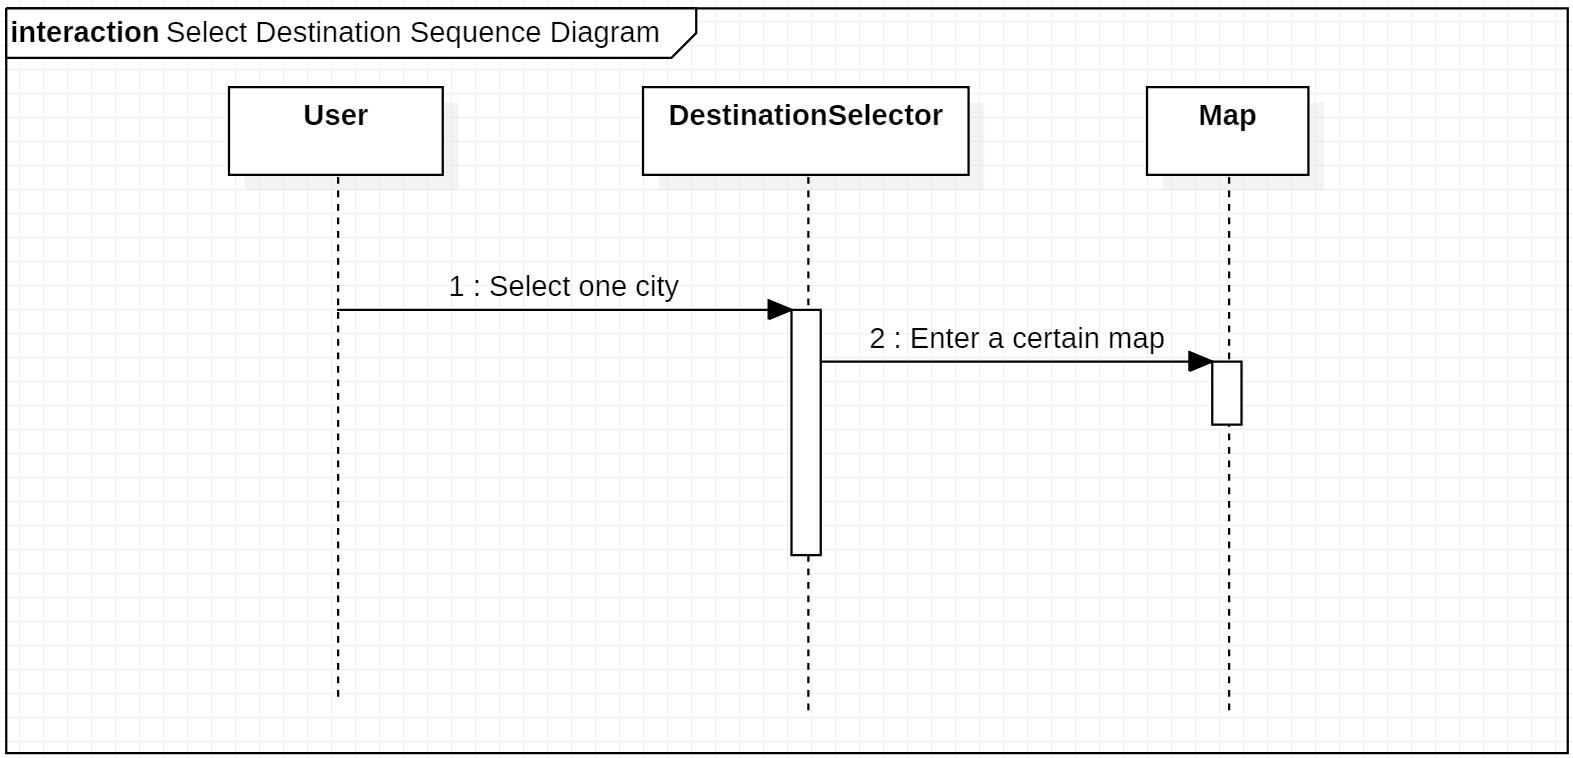
\includegraphics[width=14cm]{destination.jpg}
    \caption{Select Destination Sequence Diagram}
    \label{Select Destination Sequence Diagram}
\end{figure}

\begin{figure}[H]
    \centering
    
    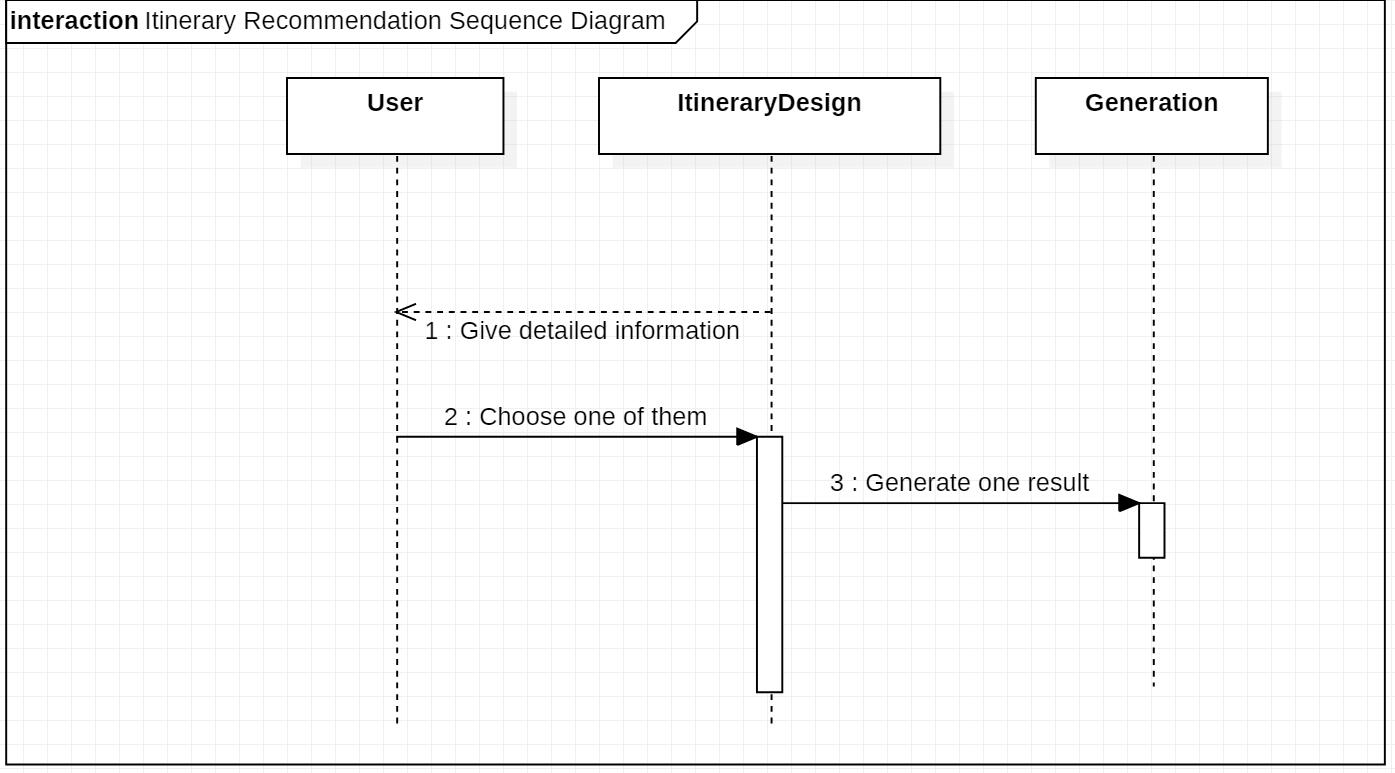
\includegraphics[width=14cm]{itinerary.jpg}
    \caption{Itinerary Recommendation Sequence Diagram}
    \label{Itinerary Recommendation Sequence Diagram}
\end{figure}

\begin{figure}[H]
    \centering
    
    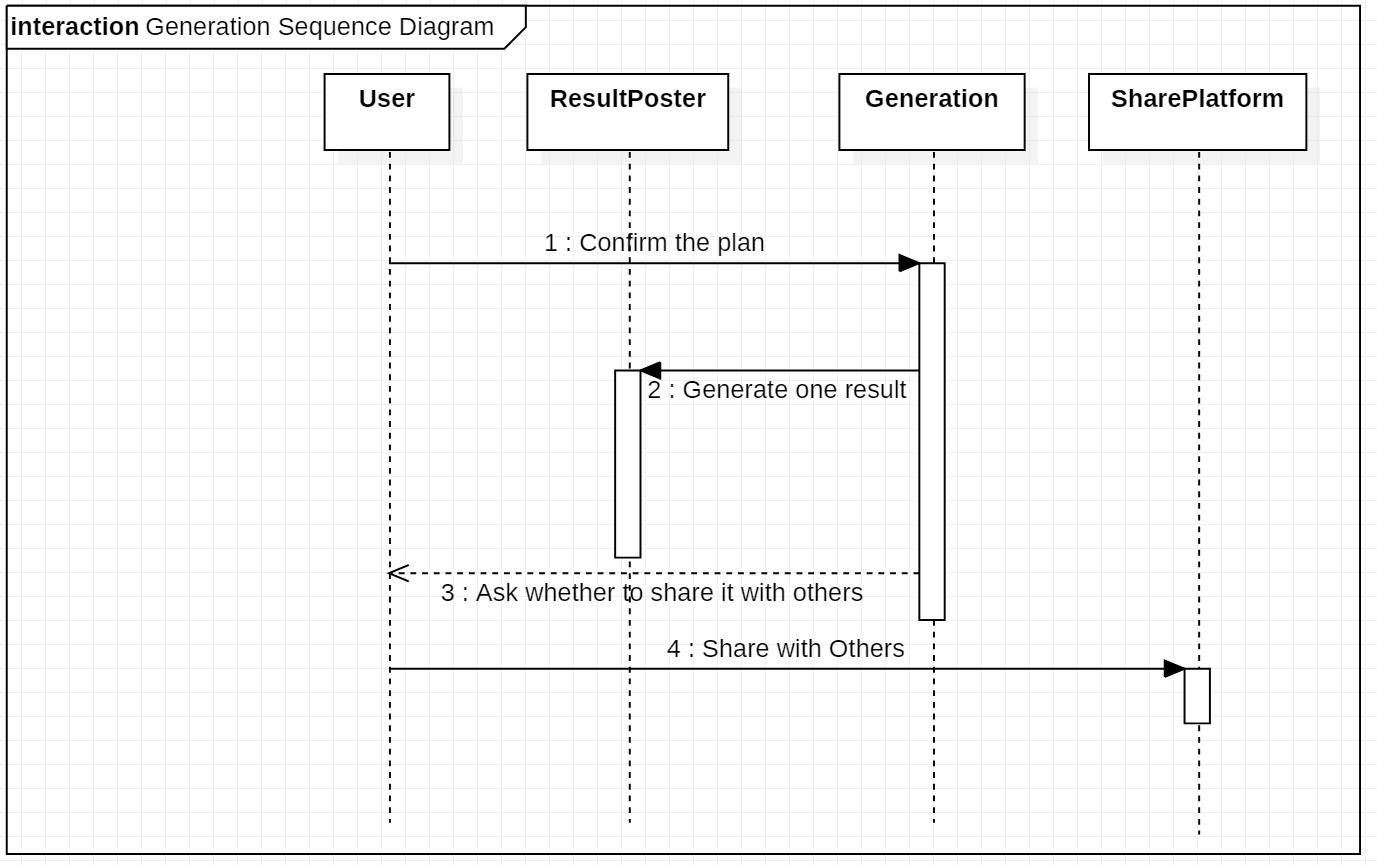
\includegraphics[width=14cm]{generation.jpg}
    \caption{Generation Sequence Diagram}
    \label{Generation Sequence Diagram}
\end{figure}

\begin{figure}[H]
    \centering
    
    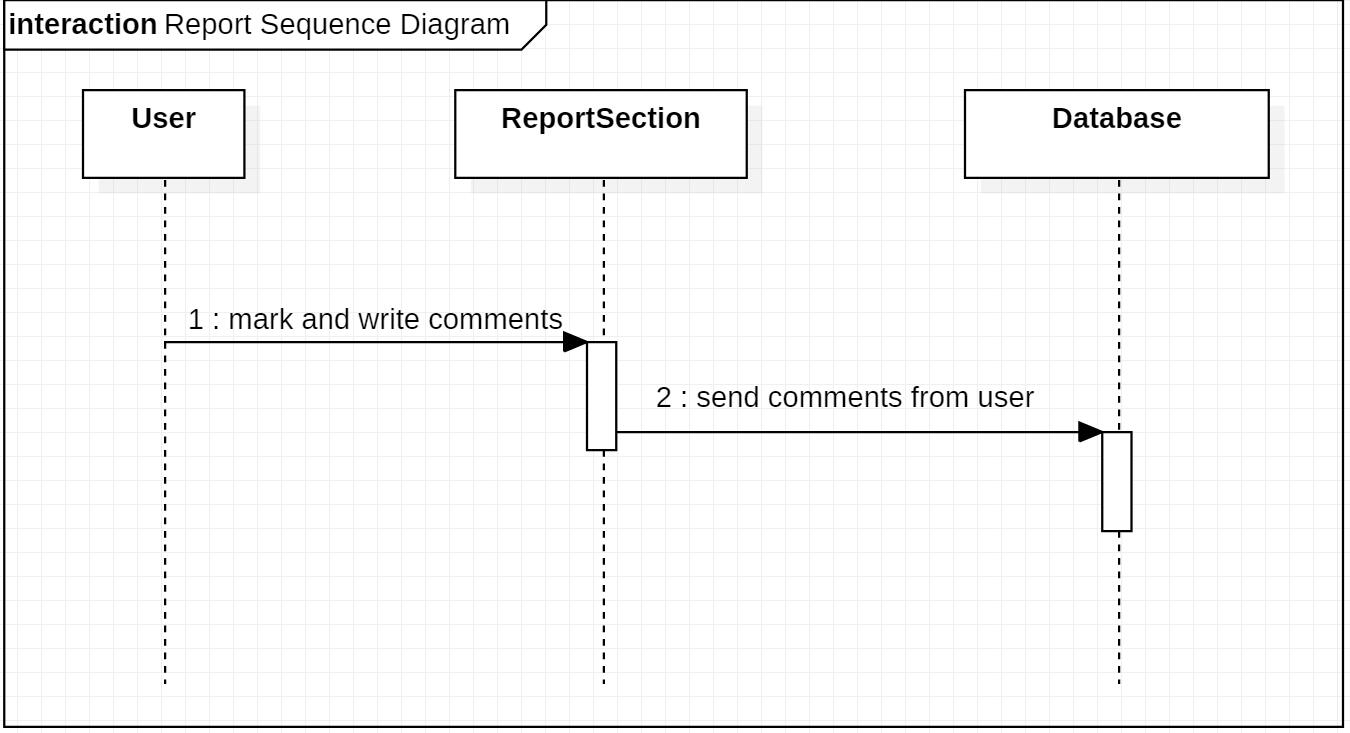
\includegraphics[width=14cm]{report.jpg}
    \caption{Report Sequence Diagram}
    \label{Report Sequence Diagram}
\end{figure}

\subsubsection{Subsystem Cooporation}

\begin{figure}[H]
    \centering
    
    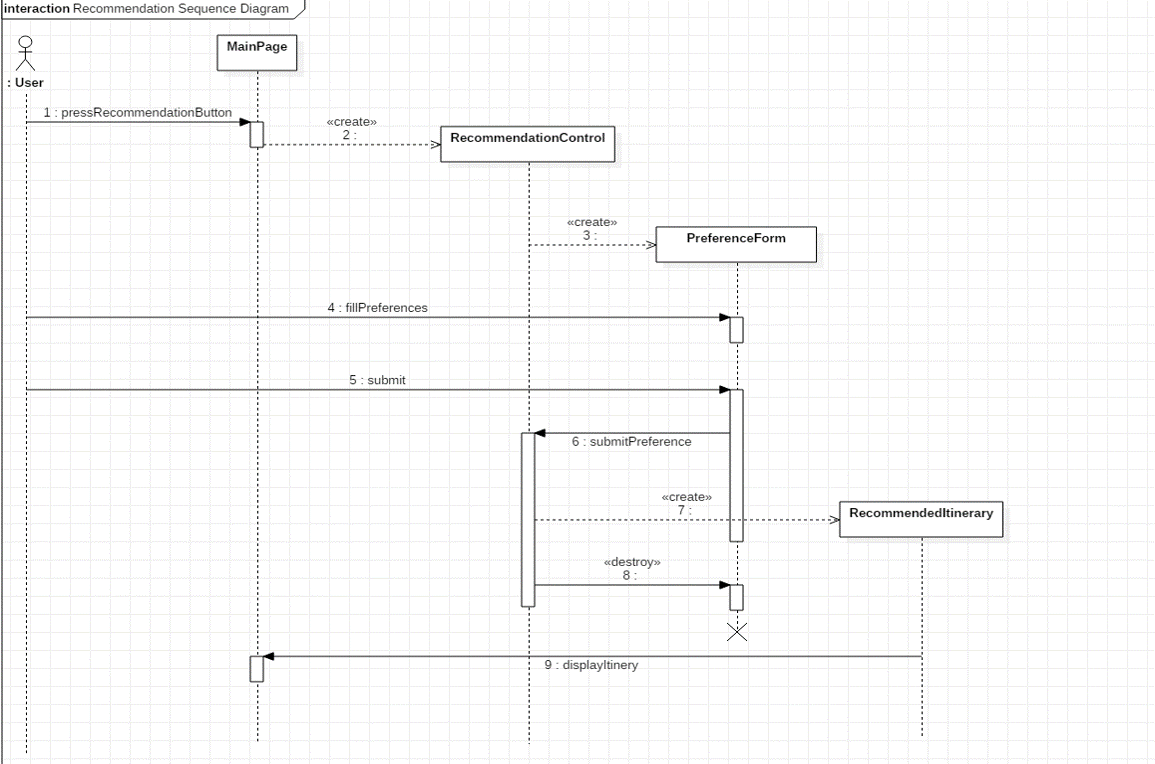
\includegraphics[width=14cm]{recommendation.png}
    \caption{Recommendation Sequence Diagram}
    \label{Recommendation Sequence Diagram}
\end{figure}

\begin{figure}[H]
    \centering
    
    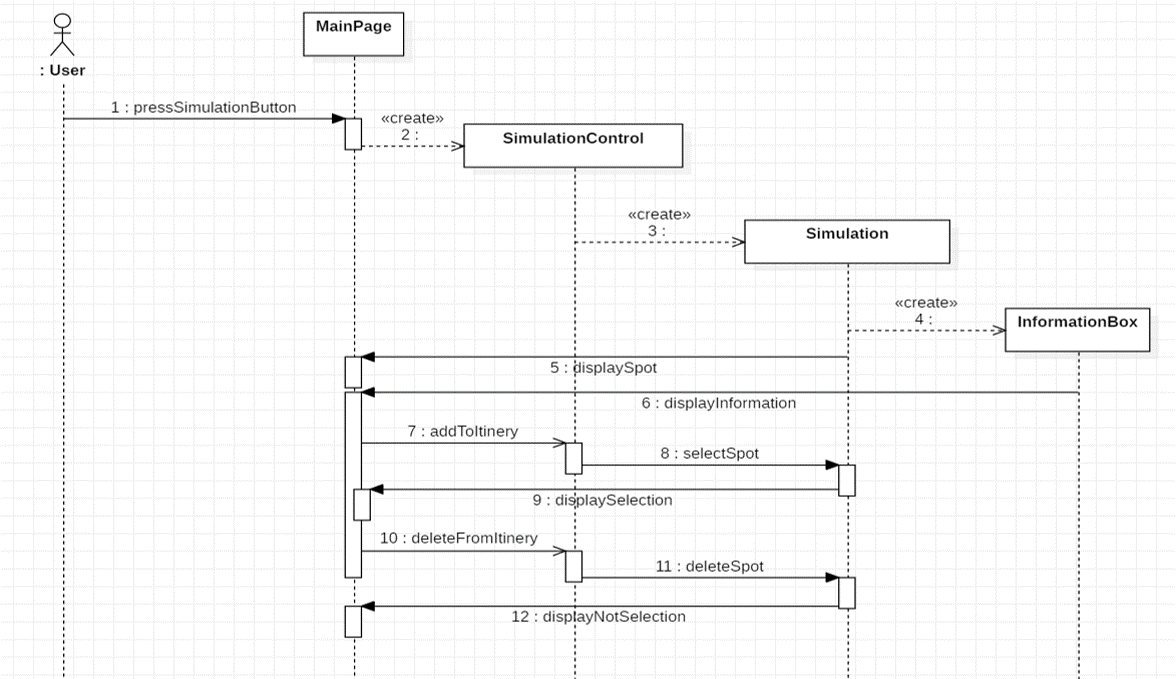
\includegraphics[width=14cm]{simulation.png}
    \caption{Simulation Sequence Diagram}
    \label{Simulation Sequence Diagram}
\end{figure}

\subsection{System Operation Diagram}
We use thread control as our control flow of our system. We split our operation diagram as Client Operation Diagram and Server Operation Diagram.

\subsubsection{Client Operation Diagram}
At the client, the UI thread is only in charge of the interaction between the system and the user. At the same time, we start a single thread for each controller and each dialog module. This kind of design can assure that the frontend, the realization of functions, and the dialog won’t collide with each other to crash our whole system.

\subsubsection{Server Operation Diagram}
At the server, for the dialog module, we will use multi-thread control to respond each client’s query. At the same time, each controller has its own thread to ensure that they won’t influence each other. For consistent service, we also use multi-thread to make the system stable.

\begin{figure}[H]
    \centering
    
    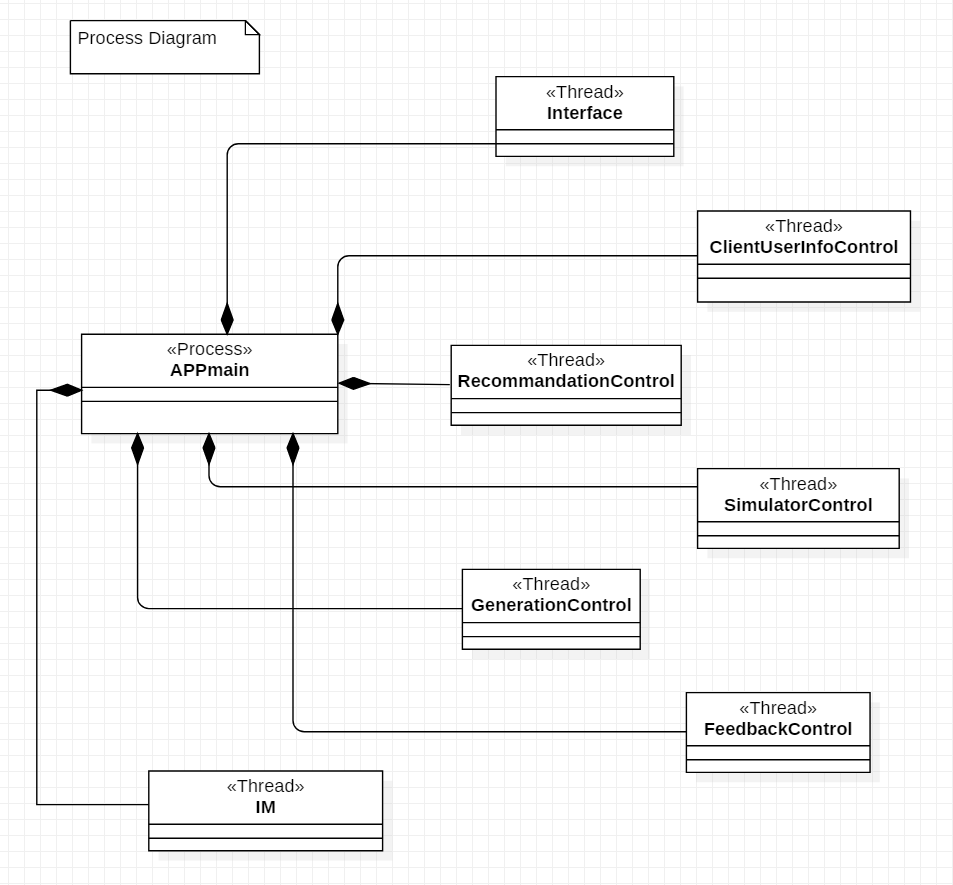
\includegraphics[width=14cm]{process.png}
    \caption{Process Diagram}
    \label{Process Diagram}
\end{figure}

\subsection{Physical View of the System}
The hardware disposition requests are as follows:

\paragraph{\underline{User Machine}} An Android device with 2GB (or more) RAM and a mainstream CPU such as Qualcomm Snapdragon and HUAWEI Kirin. Low-end phones will not face any trouble using our application.

\paragraph{\underline{Application Server}} To meet the requirement of high-density computing and data flow, we need at least 2 servers with Intel Core CPU (7-Gen or higher), 8GB (or more) memory, and 512GB (or more) storage. To be more specific, we may deploy two different kinds of hard disk: For our 'Management' server, we will use SSD to speed up the service. For the 'Database' server, we will use HDD to make sure the data is safe. Besides, the 'Management' server will be deployed with a NVIDIA GPU which supposts CUDA. It will help with machine-learning-related tasks. 

\paragraph{\underline{Network}} Take the maximum number of concurrent events as 1000. To support our system, we need 20MB exclusive bandwidth to deal with the estimated 5kb/s data flow. The exclusive bandwidth guarantee the performance of data exchange.

\subsection{Design of Boundary Condition}
We will here discuss three kinds of use cases: startup, shutdown and error handling. Detailed interaction diagrams are also present to explain how these use cases are realized. However, due to the fact that the coding job has not been finished yet, we will not discuss it in detailed. Only rough realizations will be shown here.

\subsubsection{Server Startup}
To start up the server, we need to launch a series of service that ensure our system runs persistently and all components works smoothly.

\begin{itemize}
  \item[(1)] Click the startup icon.
  \item[(2)] Initialize the object of server site 'ServerSite'.
  \item[(3)] Create the object of persistent service 'PersistentService'.
  \item[(4)] Create the objects, which will be named as 'ServerDialogControl',  'ServerDataControl' and 'ServerUserControl' respectively, to control system dialog, data and user information. These objects will refers to 'ServerSite' and 'PersistentService'.
  \item[(5)] Launch the IM (instant messaging) service, which is packed in 'IMSDK'.
\end{itemize}

\begin{figure}[H]
	\centering
	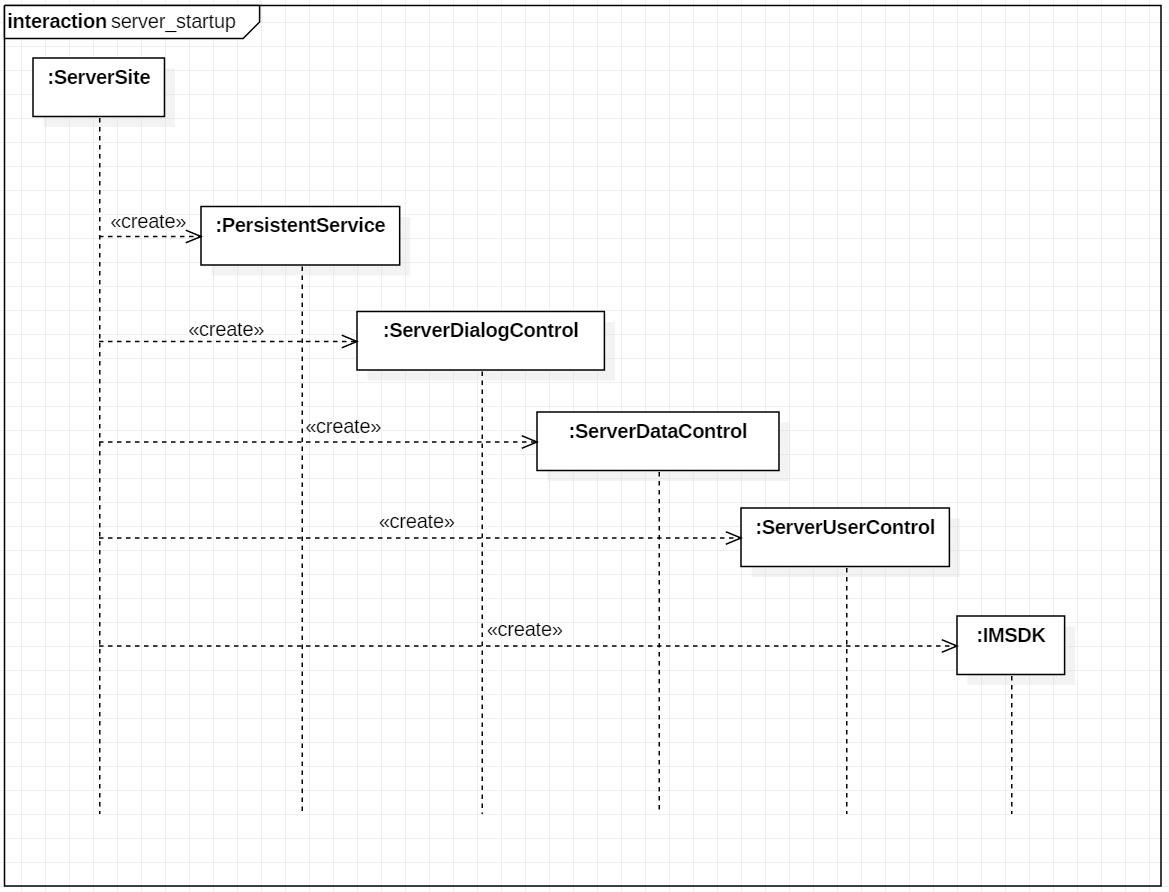
\includegraphics[width=14cm]{1.jpg} 
	\caption{Use Case Realization of 'Server Startup'}
	\label{Use Case Realization of 'Server Startup'}
\end{figure}

\subsubsection{Server Shutdown}

\begin{itemize}
	\item[(1)] Click the shutdown icon.
	\item[(2)] Delete 'ServerUserControl', 'ServerDialogControl', and 'ServerDataControl'. Close the IM service as well.
	\item[(3)] Disconnect from the database, and delete 'PersistentService'.
	\item[(4)] Delete 'ServerSite'.
\end{itemize}

\begin{figure}[H]
	\centering
	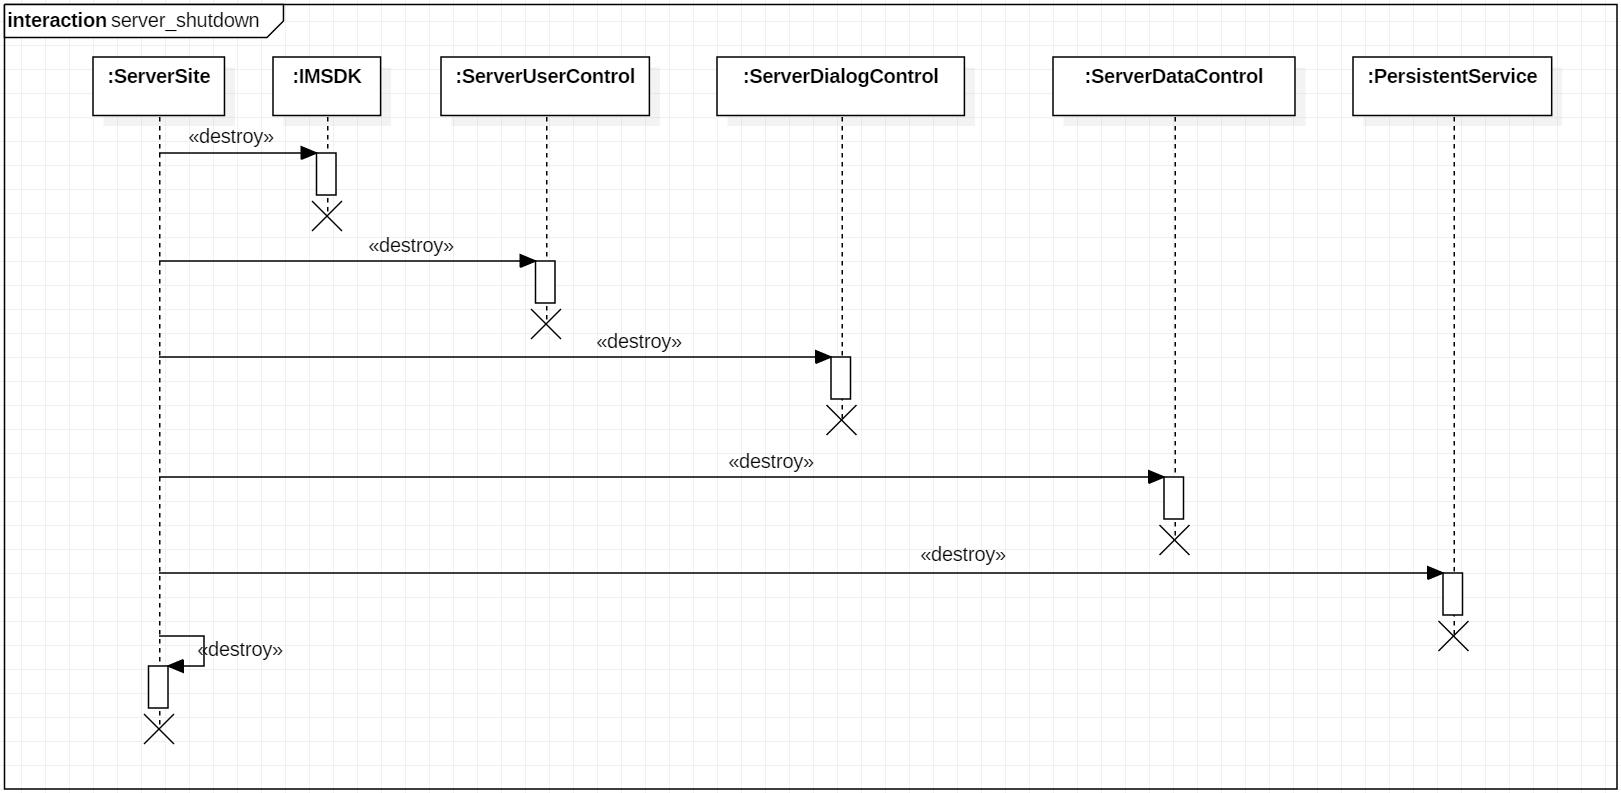
\includegraphics[width=14cm]{2.jpg} 
	\caption{Use Case Realization of 'Server Shutdown'}
	\label{Use Case Realization of 'Server Shutdown'}
\end{figure}

\subsubsection{App Startup}
To start up the application, we need to enable our system to manage different kinds of requests.

\begin{itemize}
	\item[(1)] Click the App icon.
	\item[(2)] Launch the 'MainPage' object.
	\item[(3)] The 'MainPage' object launchs 'HttpUtil' object to handle http request.
	\item[(4)] The 'MainPage' object launchs IM service.
	\item[(5)] The 'MainPage' object launchs a series of 'Adapter' objects to deal with all kinds of user request. They are 'DialogAdapter', 'DataAdapter', and 'UserAdapter', which will refer to 'HttpUtil'.
	\item[(6)] The 'MainPage' object launchs other 'ClientControl' objects to deal with further manage requests.  They are 'ClientDialogControl', 'ClientDataControl', and 'ClientUserControl', which will refer to those 'Adapter' objects. 
	\item[(7)]  The 'MainPage' object launchs 'LoginPage' object, and 'ClientUserControl' will be refered to it.
\end{itemize}

\begin{figure}[H]
	\centering
	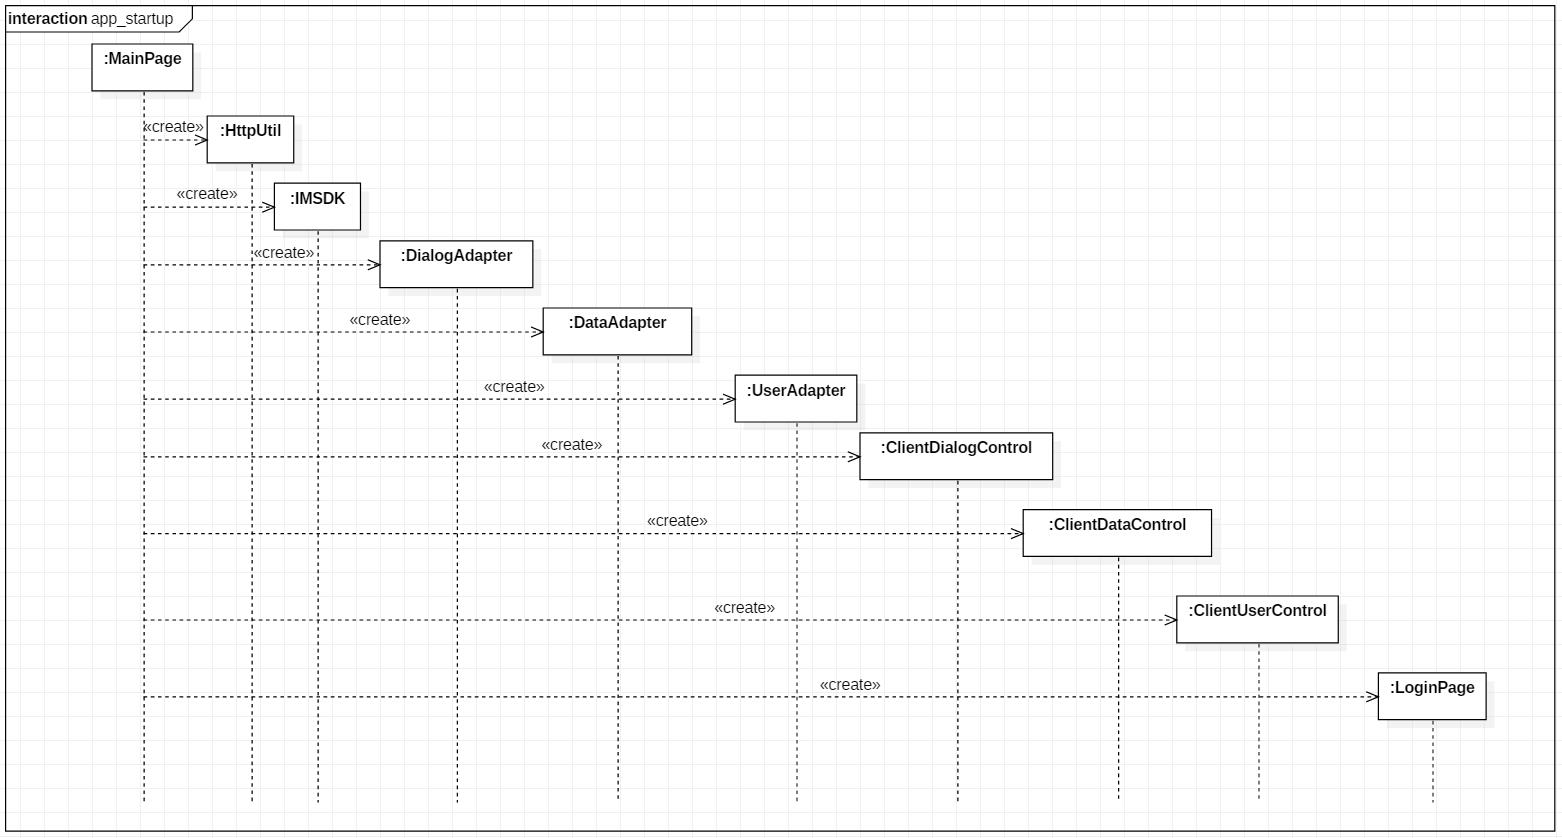
\includegraphics[width=14cm]{3.jpg} 
	\caption{Use Case Realization of 'App Startup'}
	\label{Use Case Realization of 'App Startup'}
\end{figure}

\subsubsection{App Shutdown}

\begin{itemize}
	\item[(1)] Close the App.
	\item[(2)] Delete all the 'ClientControl' objects.
	\item[(3)] Delete all the 'Adapter' objects.
	\item[(4)] Close IM service and delete 'HttpUtil'.
	\item[(5)] Delete 'MainPage'.    
\end{itemize}

\begin{figure}[H]
	\centering
	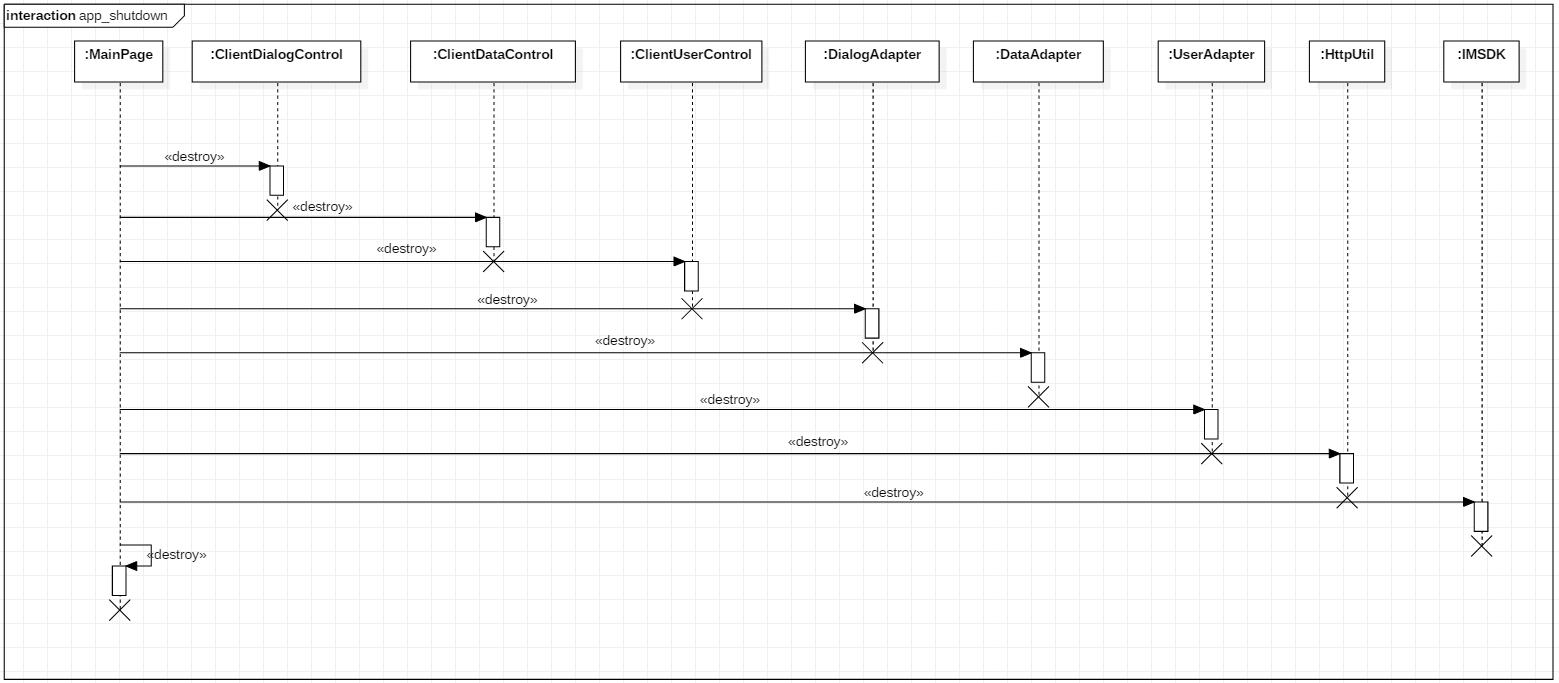
\includegraphics[width=14cm]{4.jpg} 
	\caption{Use Case Realization of 'App Shutdown'}
	\label{Use Case Realization of 'App Shutdown'}
\end{figure}

\subsubsection{Error Handling}

\begin{itemize}
	\item[(1)] If the application has an error, restart App.
	\item[(2)] If the server has an error, restart the server.
	\item[(3)] We can assume that our database is safe since nearly any database has event management system. 
\end{itemize}

\subsection{Data Management Design}
We will use relational database to manage our data. One of the reasons is that we are familiar with relational databases such as MySQL. But more than that, relational databases are better at handling massive data, comparing with some non-relational databases.

Several typical tables are present as shown here (Table \ref{UserInfo} - Table \ref{Spot}):

\begin{table}[htb]
	\centering

	\begin{tabular}{c|c|c|c|c|c|c|c} 
        \hline 
        No&Field&Description&Type&Allow\_NULL&Primary Key&Unit&Remark\\
		\hline
		1&userID&User ID&int&N&Y&&\\
		\hline
		2&userName&User Name&String&N&N&&\\
		\hline
		3&password&User Password&String&N&N&&\\
		\hline
		4&phoneNumber&User Phone Number&String&N&N&&\\
		\hline
		5&mail&User Email&String&N&N&&\\
		\hline
	\end{tabular}   
	
	\caption{UserInfo}\label{UserInfo}
\end{table}

\begin{table}[htb]
	\centering

	\begin{tabular}{c|c|c|c|c|c|c|c} 
        \hline 
        No&Field&Description&Type&Allow\_NULL&Primary Key&Unit&Remark\\
		\hline
		1&itineraryID&Itinerary ID&int&N&Y&&\\
		\hline
		2&userID&User ID&int&N&N&&\\
		\hline
	\end{tabular}   
	
	\caption{ItineraryList}\label{ItineraryList}
\end{table}

\begin{table}[htb]
	\centering

	\begin{tabular}{c|c|c|c|c|c|c|c} 
        \hline 
		No&Field&Description&Type&Allow\_NULL&Primary Key&Unit&Remark\\
		\hline
		1&itineraryID&Itinerary ID&int&N&Y&&\\
		\hline
		2&spotList&Spots on the itinerary&int&N&Y&&\\
	\end{tabular}   
	
	\caption{Itinerary}\label{Itinerary}
\end{table}

\begin{table}[htb]
	\centering

	\begin{tabular}{c|c|c|c|c|c|c|c} 
        \hline 
        No&Field&Description&Type&Allow\_NULL&Primary Key&Unit&Remark\\
		\hline
		1&spotID&Spot ID&int&N&Y&&\\
		\hline
		2&spotType&Spot Type&int&N&N&&\\
		\hline
		3&arriveTime&\tabincell{c}{Time when the user \\arrives at the spot}&time&N&N&&\\
		\hline
		4&leaveTime&\tabincell{c}{Time when the user \\leaves the spot}&time&N&N&&\\
		\hline
		5&rate&Recommendation Rate&int&N&N&&\\
		\hline
		6&description&Basic description of the spot&String&N&N&&\\
		\hline 
		7&itineraryID&Itinerary ID&int&N&Y&&\\
		\hline
	\end{tabular}   
	
	\caption{Spot}\label{Spot}
\end{table}

\begin{figure}[H]
	\centering
	
	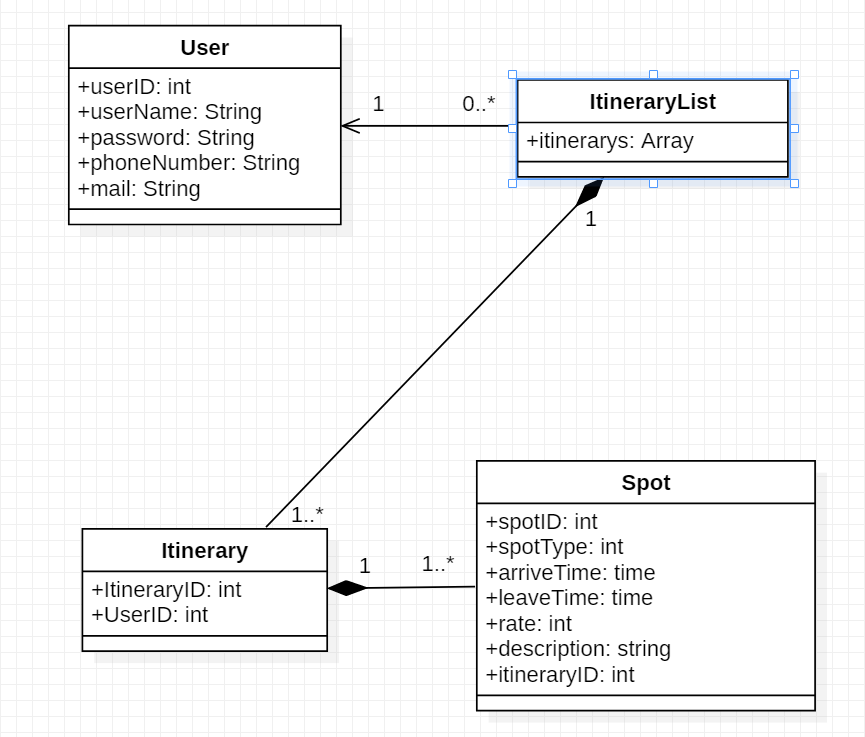
\includegraphics[width=14cm]{entity.png}
	\caption{Entity Class Design Diagram}
	\label{Entity Class Design Diagram}
\end{figure}

\subsection{Other Design}
In this part, we are going to talk something about our special designs.

\subsubsection{Access Control and Safety Design}
Logging in our system needs correct user name and password. We will match the input and our database to affirm whether it is effective. Retrieving password needs to get the verification code by origin phonenumber or e-mail address. A user who does not log in can only have limited access rights. Only the ones who log in can visit their browsing history and give a report to our system.

Table \ref{Access Control and Safety Design} shows detailed access rights after login.

\begin{table}[htb]
	\centering

	\begin{tabular}{c|c|c|c} 
		\hline
		&User Information&Itinerary&Report\\
		\hline 
		Log-in User&\tabincell{c}{Modify Information\\View History}&\tabincell{c}{Design Itinerary\\Simulation\\Recommandation}&Send User Report\\
		\hline
	\end{tabular}   
	\caption{Access Control and Safety Design}\label{Access Control and Safety Design}
\end{table}

\subsection{Reliability Design}
To make our service more nice, the feedback part will be updated monthly. That is, related database will be updated. Additionally, we will make a buck-up for the database of user’s information, in order to protect data from losing and leaking. Besides, a spare server will be equipped to deal with emergencies.

\end{document} 